\documentclass[doc,norsk]{apa7}
\usepackage[style=apa]{biblatex}
\usepackage[utf8]{inputenc}
\usepackage[norsk]{babel}
\usepackage{graphicx}
\usepackage{endfloat}

\DeclareLanguageMapping{norsk}{norsk-apa}

\bibliography{references.bib}

\title{Hvem er Institutt for Psykologis beste p-hacker?}
\shorttitle{Hvem er Institutt for Psykologis beste p-hacker?}
\author{Ole Fredrik Borgundvåg Berg}
\affiliation{NTNU}

\begin{document}

\maketitle

Replikasjonsgraden i psykologi er lav. Den mest kjente studien på området kommer fra Open Science Collaboration, som fant at når de prøvde å replikere 97 ulike psykologistuder, så klarte de kun å få signifikante resultater 36\% av replikasjonene \parencite{open-replikasjon}. Videre var effektstørrelsen i replikasjonene omtrent halvparten av de effektstørrelsen i de opprinnelige studiene. En annen studie med kun 28 replikasjoner fant en replikasjonsrate på 54\% \parencite{replikasjonsrate-2}. Det er mange ulike grunner til at replikasjonraten er lav, men en del av det kan skyldes ting som publikasjonsbias, p-hacking og liknende. Ved å se på p-verdiene i artiklene til ulike forkere kan man prøve å finne i hvilken grad p-hacking forekommer og man kan prøve å estimere i hvilken grad resultatene er forventet å replikere. I denne artikkelen skal jeg se på p-verdiene til ulike forskere ved Institutt for Psykologi. 

\subsection{Hvoran lese grafene}
Grafene er histogrammer, der dataene er z-verdier fra artiklene de har publisert. Om andre statistiske tester enn z-test er brukt, er test-statistikken omgjort til en z-verdi ved å ta z-verdien med samme p-verdi. I grafen er det en rød linje som går ved $z=1.96$. Dette er fordi en z-verdi på 1.96 eller høyere fører til en p-verdi på 0.05 eller lavere. Med andre ord, signifikante resultater er til høyre for linja og nullresultater er til venstre for linja. Det er tre tall i grafen. \guillemetleft Observed discovery rate\guillemetright\ (ODR) er andelen av de publiserte resultatene som er signifikante. \guillemetleft Expected discovery rate\guillemetright\ (EDR) er den forventede andelen signifikante resultater du vil få om du kjører alle forsøkene til forskeren på nytt. Man skulle kanskje tro at dette ville være det samme som ODR, men forskjellen er at EDR tar hensyn til seleksjonseffekter. Med spesifikt, er ODR basert på de publiserte resultatene, mens EDR tar baserer seg på alle resultatene, også de nullresultatene modellen mener finnes men ikke er blitt publisert (se avsnittet om publikasjonsbias). \guillemotleft Expected replication rate\guillemetright\ (ERR) er forventet andel signifikante resultater man vil få dersom man replikerer alle de signifikante resultatene på nytt. Det er også det som tilsvarer \guillemetleft replikasjonrate\guillemetright\ slik det er referert i første avsnitt. Mer detaljer om disse verdiene kan man finne i \textcite{z-curve-implementasjon}.

\subsection{Alexander Olsen}
\begin{figure}[h!]
    \centering
    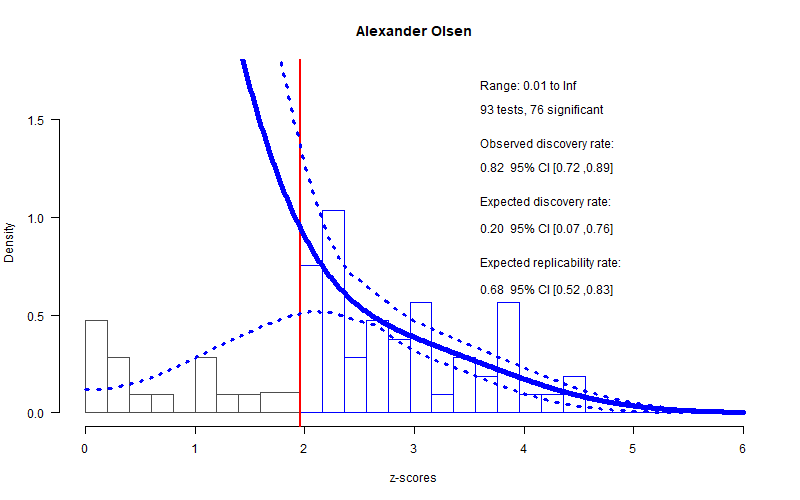
\includegraphics[width=\textwidth]{images/Alexander Olsen.png}
    \caption{z-verdier for Alexander Olsen}
\end{figure}
Alexander Olsen har en klar diskontinuetet ved $z=1.96$, noe som tyder på at det kan være en del publikasjonsbias eller p-hacking her. En forventet replikasjonsrate på 68\% er ganske OK for psykologi.

\subsection{Andrea Melanie Kessler}
\begin{figure}[h!]
    \centering
    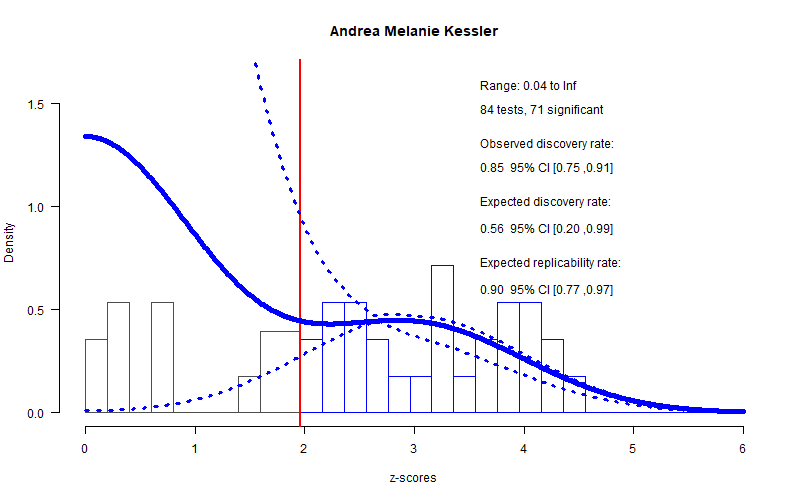
\includegraphics[width=\textwidth]{images/Andrea Melanie Kessler.png}
    \caption{z-verdier for Andrea Melanie Kessler}
\end{figure}
Andrea Melanie Kessler merker seg ved å ha en høy forventet replikasjonsrate på 90\%. Hun har heller ingen diskontinuetet ved $z=1.96$ noe som forteller oss at p-hacking eller publiseringsbias er usannsynling.

\subsection{Audrey Van der Meer}
\begin{figure}[h!]
    \centering
    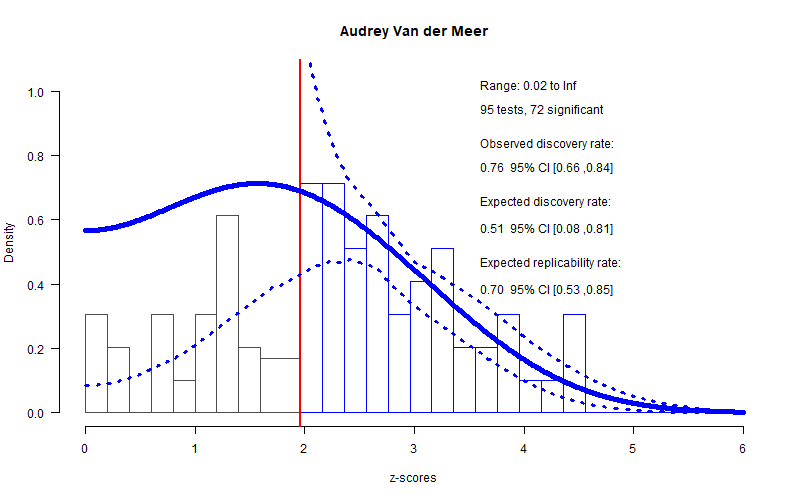
\includegraphics[width=\textwidth]{images/Audrey Van der Meer.png}
    \caption{z-verdier for Audrey Van der Meer}
\end{figure}
Audrey Van der Meer har noe diskontinuetet ved $z=1.96$, noe som kan tyde på noe p-hacking/publiseringsbias. Hun har også en forventet replikasjonsrate på 70\%, noe som er ganske OK.

% Evt: finn ut om vi skal ha med. Må i så fall legge til også hos andre med tilsvarende problemer.
% Det skal dog sies at vi fant noen p-verdier i den ene artikkelen hennes som ikke samsvarte med t-verdiene \parencite{audry-feil}. Om t-verdiene var riktige, er noen av resultatene som er rapportert som signifikante ikke faktisk signifikante.

\subsection{Audun Havnen}
\begin{figure}[h!]
    \centering
    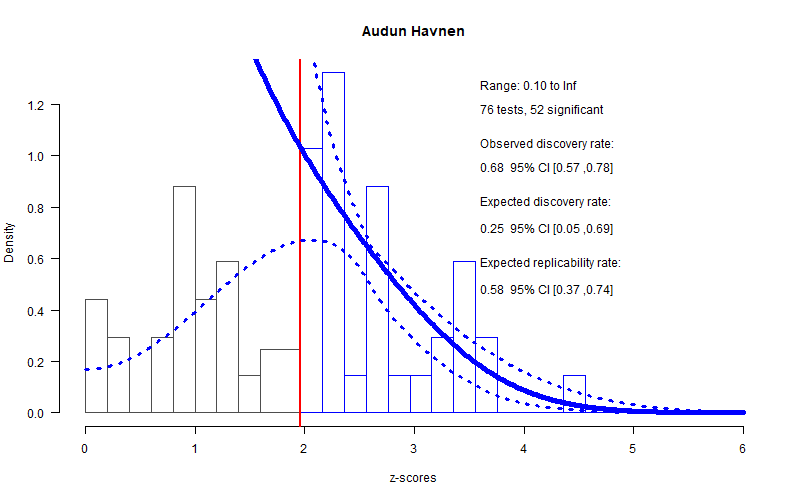
\includegraphics[width=\textwidth]{images/Audun Havnen.png}
    \caption{z-verdier for Audun Havnen}
\end{figure}
Audun Havnen har en noe lav replikasjonsrate på bare 58\%, samt en del diskontinuetet ved $z=1.96$. Dette tyder på noe p-hacking/publiseringsbias.

\subsection{Beate Wold Hygen}
\begin{figure}[h!]
    \centering
    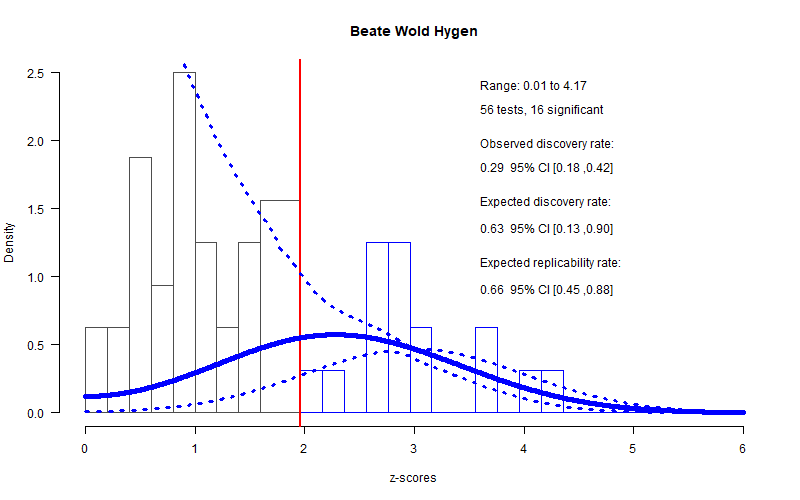
\includegraphics[width=\textwidth]{images/Beate Wold Hygen.png}
    \caption{z-verdier for Beate Wold Hygen}
\end{figure}
Beate Wold Hygen har en diskontinuetet ved $z=1.96$, men her med motsatt fortegn! Ingen p-hacking her, om noe så tyder ting på det motsatte. En forventet replikasjonrate på 66\% er også ganske bra.

\subsection{Christian Kløckner}
\begin{figure}[h!]
    \centering
    \includegraphics[width=\textwidth]{images/Christian Kløckner.png}
    \caption{z-verdier for Christian Kløckner}
\end{figure}
Christian Kløckner har en solid z-verdi-graf. Ingen diskontinuetet og mange null-resultater. En høy forventet replikasjonrate på hele 89\% er også til å legge merke til.

\subsection{Dawn Marie Behne}
\begin{figure}[h!]
    \centering
    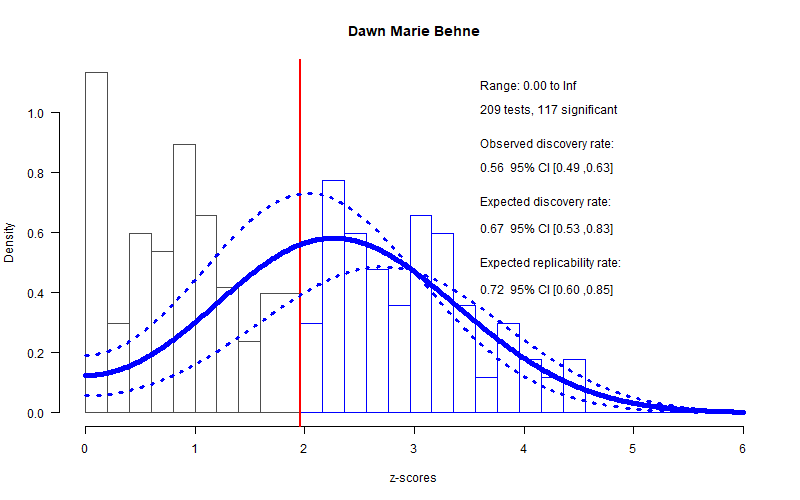
\includegraphics[width=\textwidth]{images/Dawn Marie Behne.png}
    \caption{z-verdier for Dawn Marie Behne}
\end{figure}
Dawn Marie Behne har ingen diskontinuetet ved $z=1.96$ og en helt OK forventet replikasjonrate på 72\%. Ingen tegn til p-hacking eller publiseringsbias.

\subsection{Frederick Anyan}
\begin{figure}[h!]
    \centering
    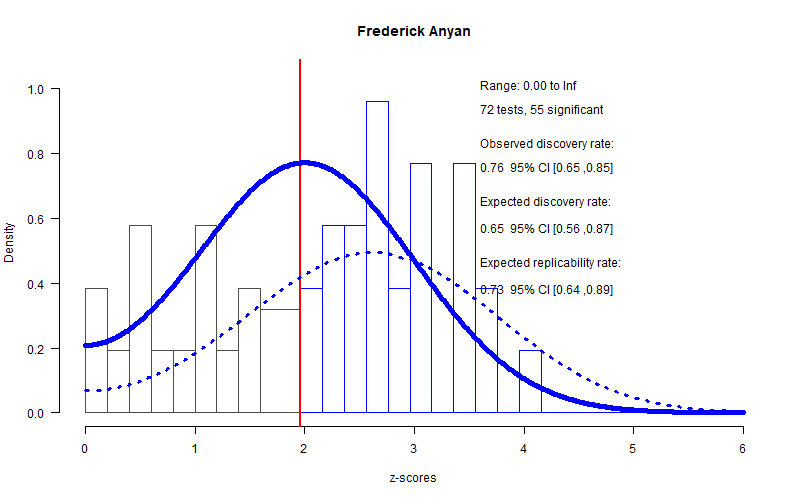
\includegraphics[width=\textwidth]{images/Frederick Anyan.png}
    \caption{z-verdier for Frederick Anyan}
\end{figure}
Frederick Anyan har en helt OK z-verdi-graf. Ingen store diskontinueteter og en forventet replikasjonrate på 73\%.

\subsection{Frederikus Van der Weel}
\begin{figure}[h!]
    \centering
    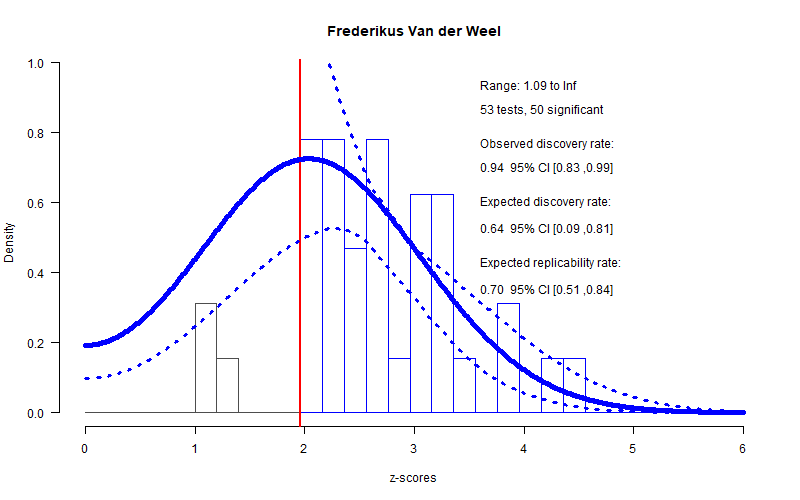
\includegraphics[width=\textwidth]{images/Frederikus Van der Weel.png}
    \caption{z-verdier for Frederikus Van der Weel}
\end{figure}
Frederick Van der Weel har den største diskontinueteten av alle i sin z-verdi-graf. Det snek seg dog med noen få nullresultater innimellom. Forventet replikasjonsraten på 70\% er ganske OK, da.

\subsection{Gerit Pfuhl}
\begin{figure}[h!]
    \centering
    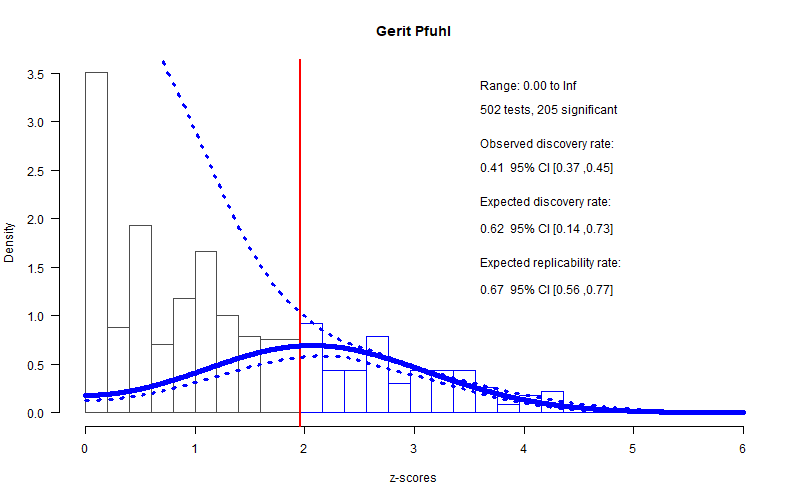
\includegraphics[width=\textwidth]{images/Gerit Pfuhl.png}
    \caption{z-verdier for Gerit Pfuhl}
\end{figure}
Gerit Pfuhl har klart å unngå diskontinueteter i sin graf og har mange null-resultater. En forventet replikasjonrate på 67\% er ganske grei. Man begynner dog å se konturene av en gausskurve i z-verdi-grafen hennes, noe som gjør at man kan begynne å lure på om det er nullhypotesen som er i grafen her.

\subsection{Hermundur Sigmundsson}
\begin{figure}[h!]
    \centering
    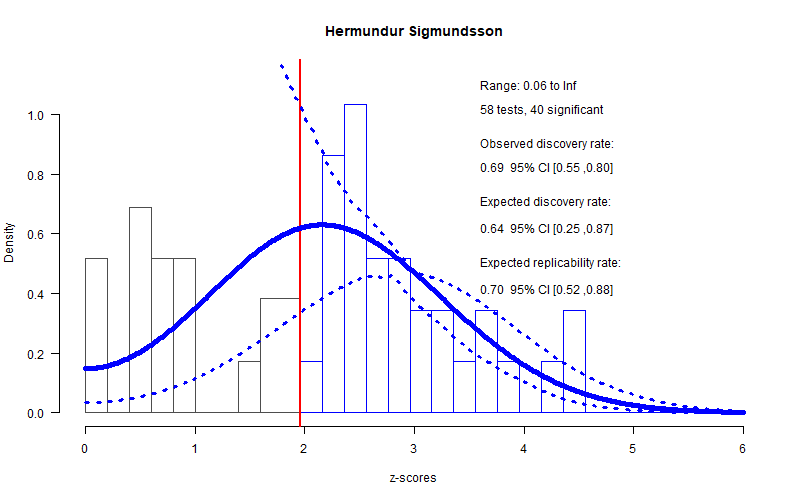
\includegraphics[width=\textwidth]{images/Hermundur Sigmundsson.png}
    \caption{z-verdier for Hermundur Sigmundsson}
\end{figure}
Hermundur Sigmundsson har noe diskontinuetet ved $z=1.96$, men det er også en god del null-resultater. Den forventede replikasjonraten på 70\% er også ganske OK.

\subsection{Ida Emilia Brunner}
\begin{figure}[h!]
    \centering
    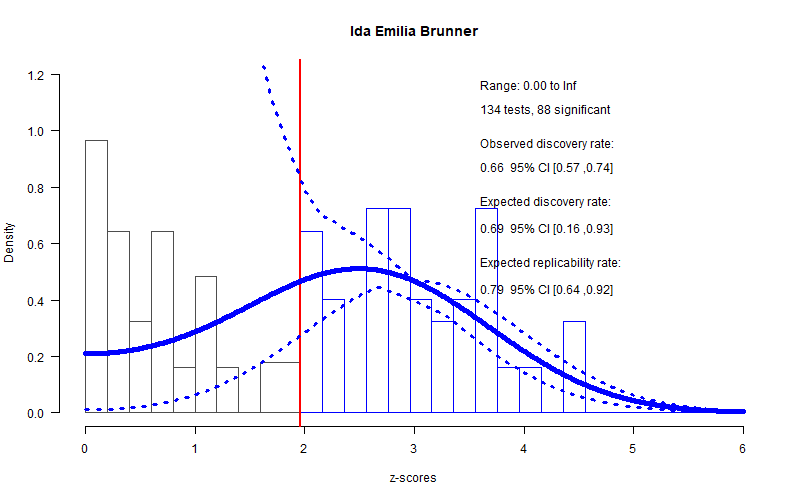
\includegraphics[width=\textwidth]{images/Ida Emilia Brunner.png}
    \caption{z-verdier for Ida Emilia Brunner}
\end{figure}
Ida Emilia Brunner har en ganske høy forventet replikasjonrate på 79\% og litt diskontinuetet ved $z=1.96$, men det er også en god del null-resultater.

\subsection{Ingvild Saksvik-Lehouillier}
\begin{figure}[h!]
    \centering
    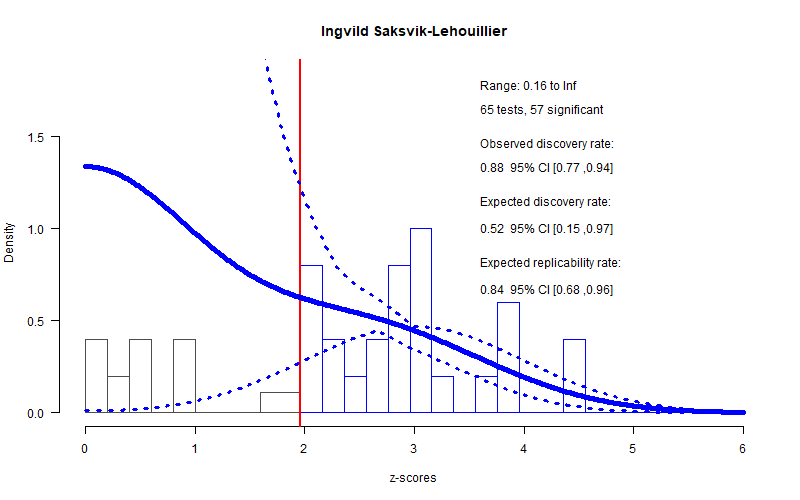
\includegraphics[width=\textwidth]{images/Ingvild Saksvik-Lehouillier.png}
    \caption{z-verdier for Ingvild Saksvik-Lehouillier}
\end{figure}
Ingvild Saksvik-Lehouillier sin forsking vil replikeres i 84\% av tilfellene i følge modellen, noe som er ganske bra. Skal sies at det er en viss diskontinuetet ved $z=1.96$, noe som gjør at det kan være noe p-hacking eller publiseringsbias.

\subsection{Jolene Van der Kaap-Deeder}
\begin{figure}[h!]
    \centering
    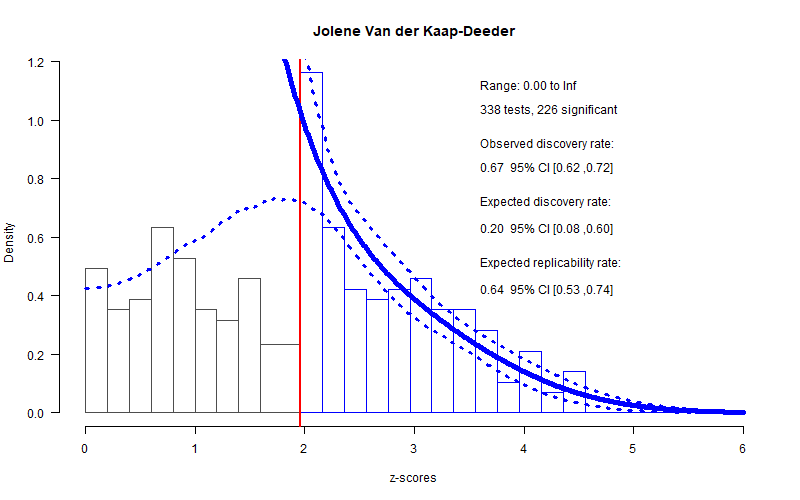
\includegraphics[width=\textwidth]{images/Jolene Van der Kaap-Deeder.png}
    \caption{z-verdier for Jolene Van der Kaap-Deeder}
\end{figure}
Jolene Van der Kaap-Deeder har en veldig gausskurve-form på funnene hennes på høyresiden av $z=1.96$, men denne stopper helt opp. Dette kan tyde på noe manglende nullresultater, men det er også en del nullresultater i grafen hennes. Den forventede replikasjonraten på $64\%$ er noe lavt i forhold til andre her.

\subsection{Lars Wichstrøm}
\begin{figure}[h!]
    \centering
    \includegraphics[width=\textwidth]{images/Lars Wichstrøm.png}
    \caption{z-verdier for Lars Wichstrøm}
\end{figure}
Lars Wichstrøm har en helt OK z-verdi-graf. Ingen store diskontinueteter og en replikasjonsrate på 71\%. Har med en grei andel nullresultater.

\subsection{Leif Edward Ottesen Kennair}
\begin{figure}[h!]
    \centering
    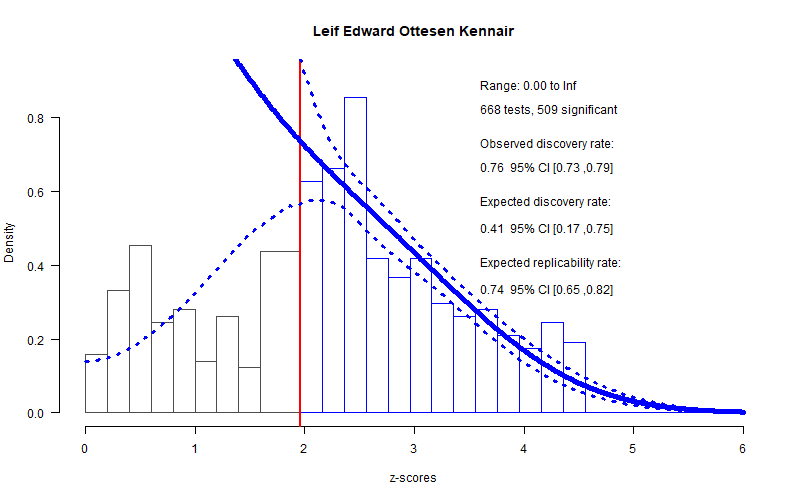
\includegraphics[width=\textwidth]{images/Leif Edward Ottesen Kennair.png}
    \caption{z-verdier for Leif Edward Ottesen Kennair}
\end{figure}
Leif Edward Ottesen Kennair har en viss diskontinuetet ved $z=1.96$, men den er ikke så stor. Likevel, hvis man ser på trenden på høyresiden av $z=1.96$ så kan man tro at det er en del manglende nullresultater her, siden trenden mistenkelig nok snur der den gjør. Forventet replikasjonrate er på relativt greie 74\%. Såvidt under (men ikke signifikant forskjellig fra) hans store forbilde David M. Buss på 76\% \parencite{z-curve-david-buss}.

\subsection{Magne Arve Flaten}
\begin{figure}[h!]
    \centering
    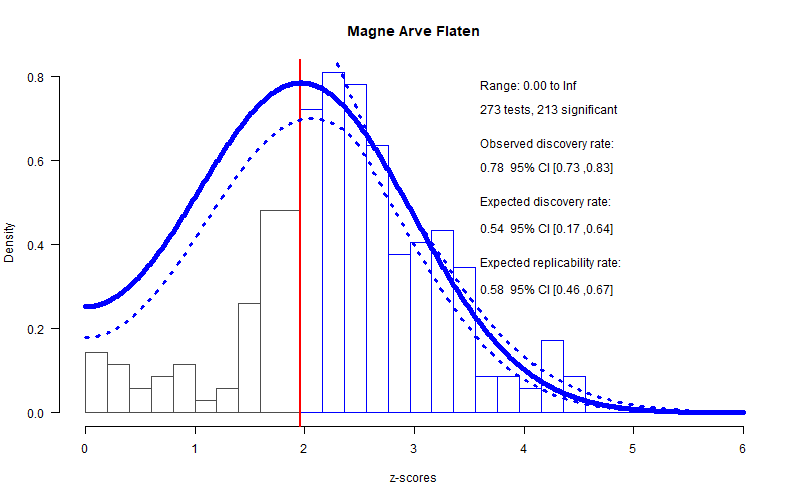
\includegraphics[width=\textwidth]{images/Magne Arve Flaten.png}
    \caption{z-verdier for Magne Arve Flaten}
\end{figure}
Magne Arve Flaten har en fin gausskurve i sin z-verdi-graf, bare at den er er sentrert rundt $z \approx 2.3$ i steden for $z = 0$ som ved nullhypotesen. Diskontinueteten ved $z = 1.96$ er ikke så stor at noe nødvendigvis er galt her. I praksis er det to muligheter her; enten så er han veldig god på styrkeanalyse eller så er det noen manglende nullresultater her. Forventet replikasjonrate er på 58\%, noe som ganske lavt i forhold til kollegaer.

\subsection{Magnus Alm}
\begin{figure}[h!]
    \centering
    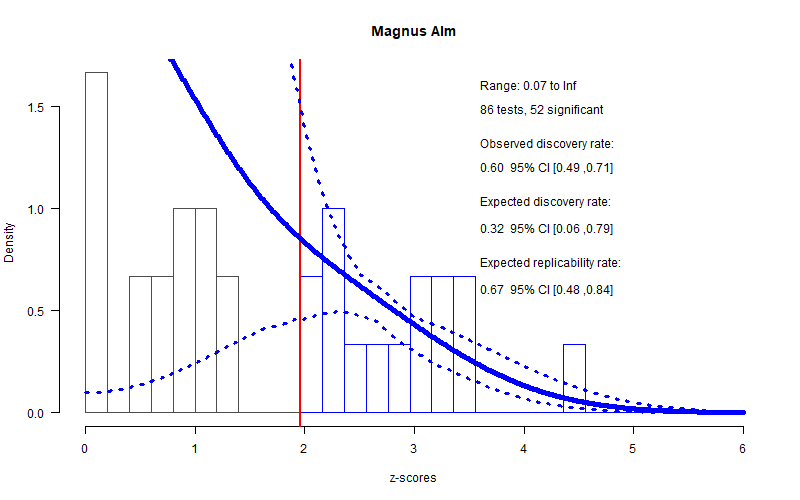
\includegraphics[width=\textwidth]{images/Magnus Alm.png}
    \caption{z-verdier for Magnus Alm}
\end{figure}
Magnus Alm har en helt OK z-verdi-graf. Litt få z-verdier her, noe som gjør det vanskelig å si noe sikkert. Ingen store diskontinuiteter, og en ganske grei forventet replikasjonrate på 67\%. En slags kontur av en gausskurve kan skimtes.

\subsection{Matthias Mittner}
\begin{figure}[h!]
    \centering
    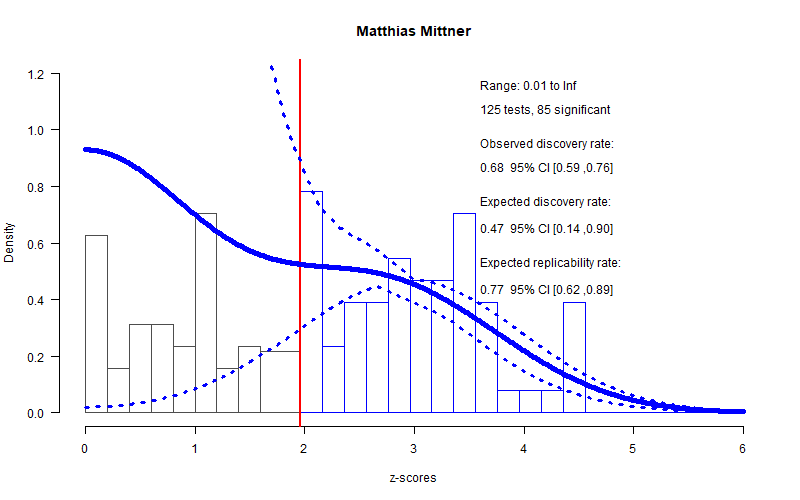
\includegraphics[width=\textwidth]{images/Matthias Mittner.png}
    \caption{z-verdier for Matthias Mittner}
\end{figure}
Matthias Mittner har en ganske flat z-verdi-graf. Ingen store diskontinueteter, men kan se ut som nivået på nullresultater er noe laver enn signifikante resultater. Mulig noen manglende nullresultater. Forventet replikasjonrate er på 77\% som er ganske bra.

\subsection{Mons Bendixen}
\begin{figure}[h!]
    \centering
    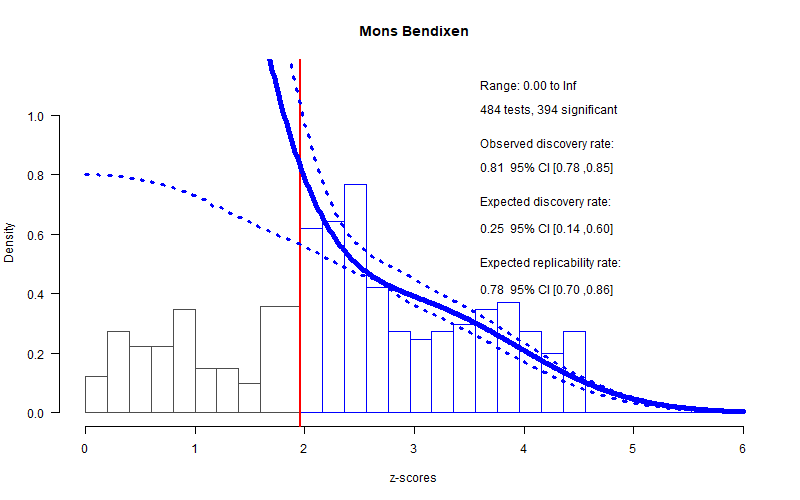
\includegraphics[width=\textwidth]{images/Mons Bendixen.png}
    \caption{z-verdier for Mons Bendixen}
\end{figure}
Mons Bendixen har noe diskontinuitet ved $z=1.96$. På høyresiden av $z=1.96$ er det konturene til en gausskurve, men den forsvinner på venstresiden, noe som kan tyde på noen manglende nullresultater her. Forventet replikasjonsrate på 78\% må sies å være ganske bra.


\subsection{Nicholas Hagen Kirkerud}
\begin{figure}[h!]
    \centering
    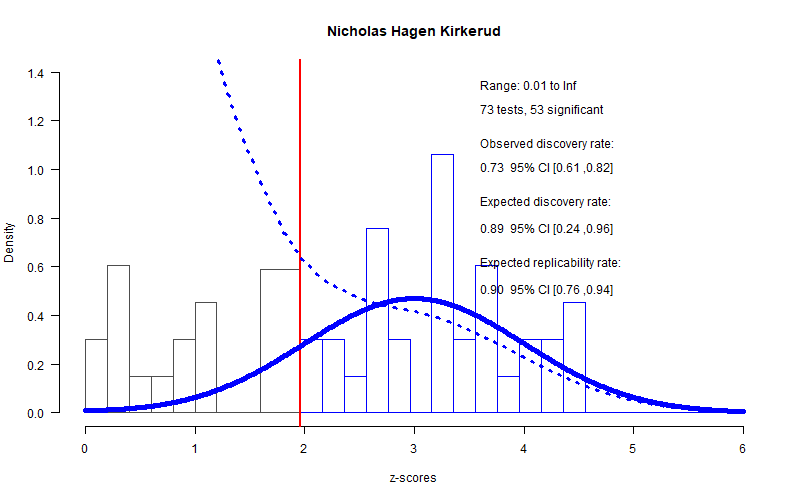
\includegraphics[width=\textwidth]{images/Nicholas Hagen Kirkerud.png}
    \caption{z-verdier for Nicholas Hagen Kirkerud}
\end{figure}
Nicholas Haugen Kirkerud har en ganske flat z-verdi-graf, men ganske få z-verdier her, så det er vanskelig å si noe sikkert. Forventet replikasjonrate på 90\% er veldig bra!

\subsection{Nunne Englund}
\begin{figure}[h!]
    \centering
    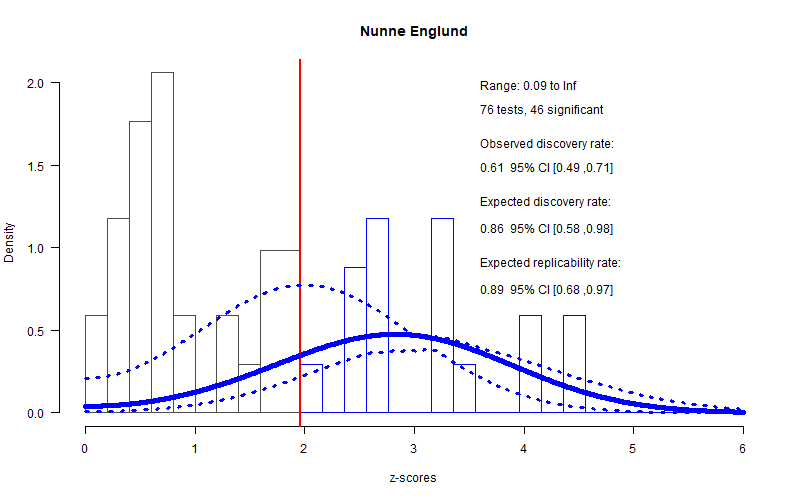
\includegraphics[width=\textwidth]{images/Nunne Englund.png}
    \caption{z-verdier for Nunne Englund}
\end{figure}
Nunne Englund har også en ganske flat z-verdi graf med få z-verdier, noe som skaper noe usikkerhet her. Skal sies at forventet replikasjonsrate er på veldig solide $89\%$!

\subsection{Odin Hjemdal}
\begin{figure}[h!]
    \centering
    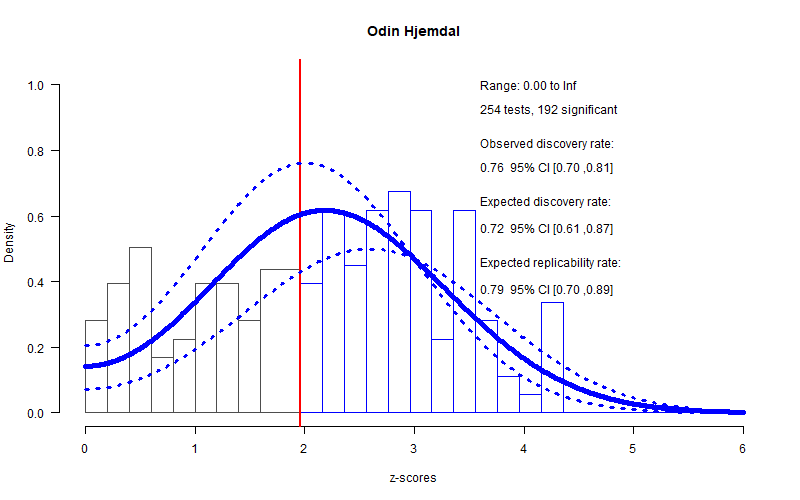
\includegraphics[width=\textwidth]{images/Odin Hjemdal.png}
    \caption{z-verdier for Odin Hjemdal}
\end{figure}
Odin Hjemdal har en grei replikasjonrate på 79\%. Ingen store diskontinueteter og grafen er relativt flat. Det skal sies at nivået på venstresiden av $z=1.96$ er noe lavere enn på høyresiden, noe som kan tyde på noen manglende nullresultater.

\subsection{Patrick A. Vogel}
\begin{figure}[h!]
    \centering
    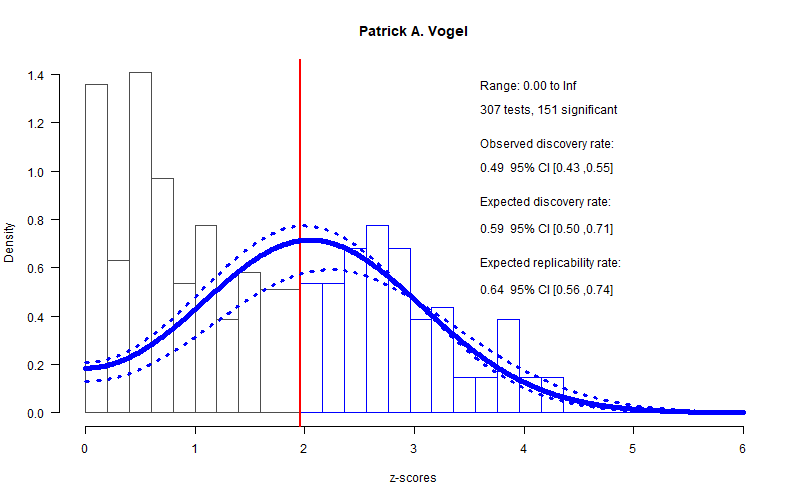
\includegraphics[width=\textwidth]{images/Patrick A. Vogel.png}
    \caption{z-verdier for Patrick A. Vogel}
\end{figure}
Patrick A. Vogel har ingen diskontinuitet ved $z=1.96$ og har en liten tendens til en gausskurve. Forventet replikasjonrate på 64\% er noe lavt i forhold til andre her, men også lite som tyder på p-hacking/publiseringsbias.

\subsection{Roger Hagen}
\begin{figure}[h!]
    \centering
    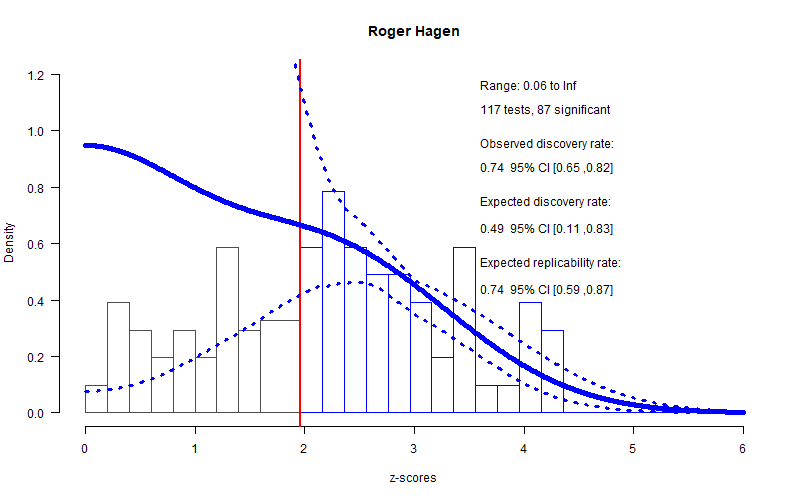
\includegraphics[width=\textwidth]{images/Roger Hagen.png}
    \caption{z-verdier for Roger Hagen}
\end{figure}
Roger Hagen har noe diskontinuitet ved $z=1.96$ som tyder på noen manglende nullresultater. Forventet replikasjonsgrad på 74\% er ganske grei.

\subsection{Stian Solem}
\begin{figure}[h!]
    \centering
    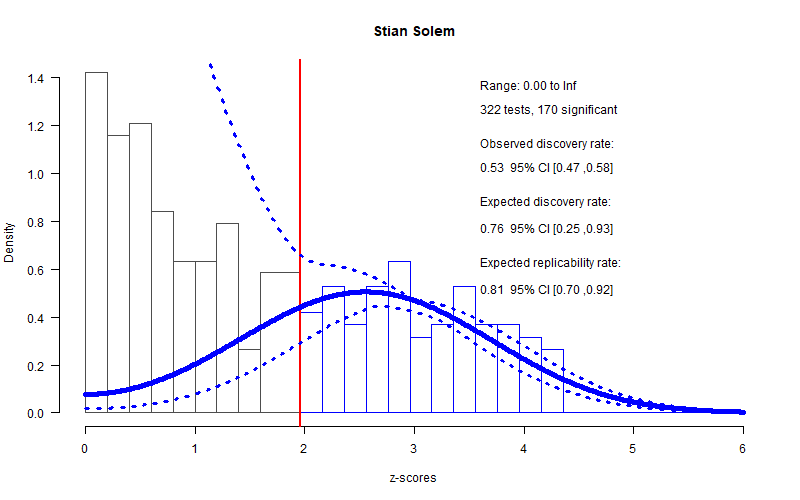
\includegraphics[width=\textwidth]{images/Stian Solem.png}
    \caption{z-verdier for Stian Solem}
\end{figure}
Stian Solem har en ganske god forventet replikasjonsrate på 81\% og heller ingen diskontinuiteter i grafen, noe som tyder på liten grad av p-hacking/publiseringsbias. Dog skal det sies at man ser en tendens til en gausskurve, noe som kan få en til å lure på i hvilken grad det er nullhypotesen vi ser grafen til her.

\subsection{Tilmann von Soest}
\begin{figure}[h!]
    \centering
    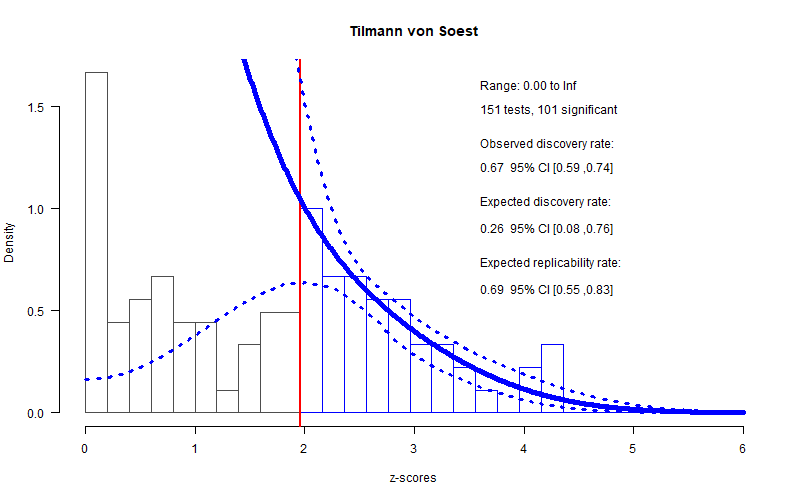
\includegraphics[width=\textwidth]{images/Tilmann von Soest.png}
    \caption{z-verdier for Tilmann von Soest}
\end{figure}
Tilmann von Soest har noe diskontinuitet ved $z=1.96$, der man ser konturene til en gausskurve på høyresiden av $z=1.96$, men denne forsvinner helt på venstresiden. Dette kan tyde på noe manglende nullresultater. Den forventede replikasjonsgraden på 69\% er ganske grei.

\subsection{Timo Juhani Lajunen}
\begin{figure}[h!]
    \centering
    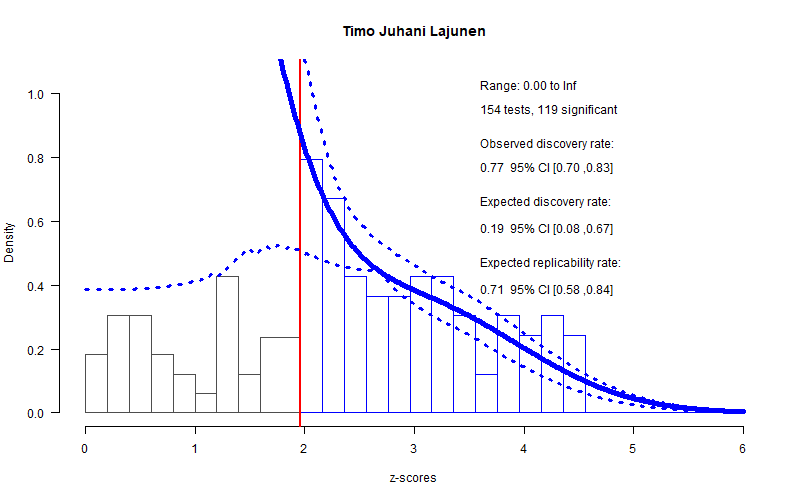
\includegraphics[width=\textwidth]{images/Timo Juhani Lajunen.png}
    \caption{z-verdier for Timo Juhani Lajunen}
\end{figure}
Timo Juhani Lajunen har en forventet replikasjonrate på 71\%, noe som er ganske OK. Når det kommer til diskontinuiteter, er diskontinuiteten ganske stor ved $z=1.96$. Man ser konturene til en gausskurve på høyre side av $z=1.96$, men ingenting slikt på venstresiden av grafen. Det kan tyde på en del manglende nullresultater, og man kan spørre seg om man bare ser nullhypotesen og publiseringsbias her.

\subsection{Tor Sunde}
\begin{figure}[h!]
    \centering
    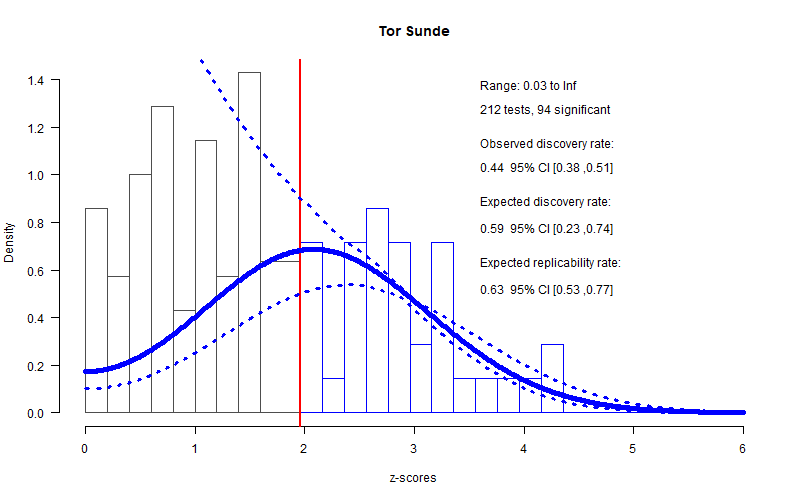
\includegraphics[width=\textwidth]{images/Tor Sunde.png}
    \caption{z-verdier for Tor Sunde}
\end{figure}
Man ser ingen diskontinuetet i grafen til Tor Sunde, noe som tyder på liten grad av p-hacking/publiseringsbias. Forventet replikasjonrate på $63\%$ er litt lavt, dog.

\subsection{Torbjørn Rundmo}
\begin{figure}[h!]
    \centering
    \includegraphics[width=\textwidth]{images/Torbjørn Rundmo.png}
    \caption{z-verdier for Torbjørn Rundmo}
\end{figure}
Torbjørn Rundmo har en av de største diskontinuitetene vi har sett ved $z=1.96$ (kun slått at Frederikus Van der Weel), med mange manglende nullresultater. Mens 94\% av hans publiserte resultater var signifikante, antar modellen at kun 25\% av de faktisk utførte forsøkene var signifikante. Det skal dog sies at han har en forventet replikasjonrate på 81\%, noe som er ganske bra.

\subsection{Tore C Stiles}
\begin{figure}[h!]
    \centering
    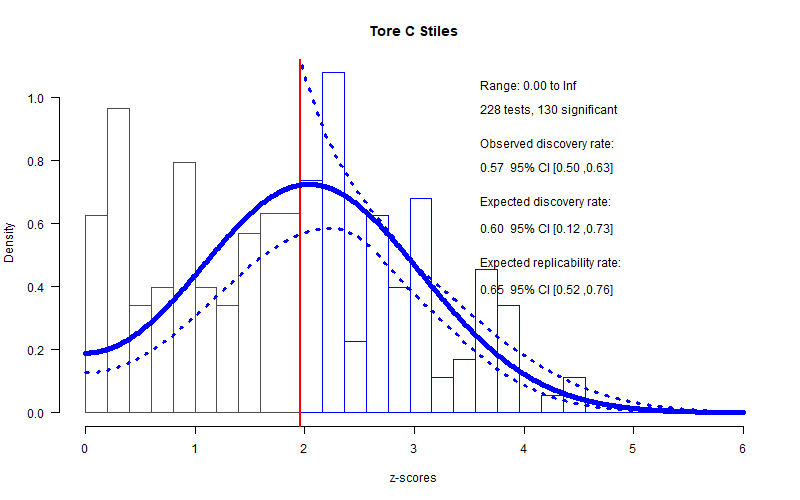
\includegraphics[width=\textwidth]{images/Tore C Stiles.png}
    \caption{z-verdier for Tore C Stiles}
\end{figure}
Tore C Stiles har en litt lav forventet replikasjonsrate på 65\%. Det er også noe diskontinuitet ved $z=1.96$ på den måten at det er en trendendring der. Det kan være at det skyldes manglende resultater, men kan også være at det skyldes god styrkeanalyse.

\subsection{Torun Grøtte}
\begin{figure}[h!]
    \centering
    \includegraphics[width=\textwidth]{images/Torun Grøtte.png}
    \caption{z-verdier for Torun Grøtte}
\end{figure}
Torun Grøtte har ingen diskontinuiteter i grafen og en god del publiserte nullresultater. På en annen side er den forventede replikasjonraten på 55\% ganske lav i forhold til kollegaer.

\subsection{Trond Nordfjærn}
\begin{figure}[h!]
    \centering
    \includegraphics[width=\textwidth]{images/Trond Nordfjærn.png}
    \caption{z-verdier for Trond Nordfjærn}
\end{figure}
Trond Nordfjærn har lite diskontinuitet i grafen sin og en ganske god forventet replikasjonsrate på 84\%.

\subsection{Trond Viggo Grøntvedt}
\begin{figure}[h!]
    \centering
    \includegraphics[width=\textwidth]{images/Trond Viggo Grøntvedt.png}
    \caption{z-verdier for Trond Viggo Grøntvedt}
\end{figure}
Trond Viggo Grøntvedt har en ganske grei forventet replikasjonsrate på 67\% og en god del publiserte nullresultater. Likevel er det en viss diskontinuitet ved $z=1.96$ ved at trenden snur, noe som kan tyde på noen manglende nullresultater.

\subsection{Ute Gabriel}
\begin{figure}[h!]
    \centering
    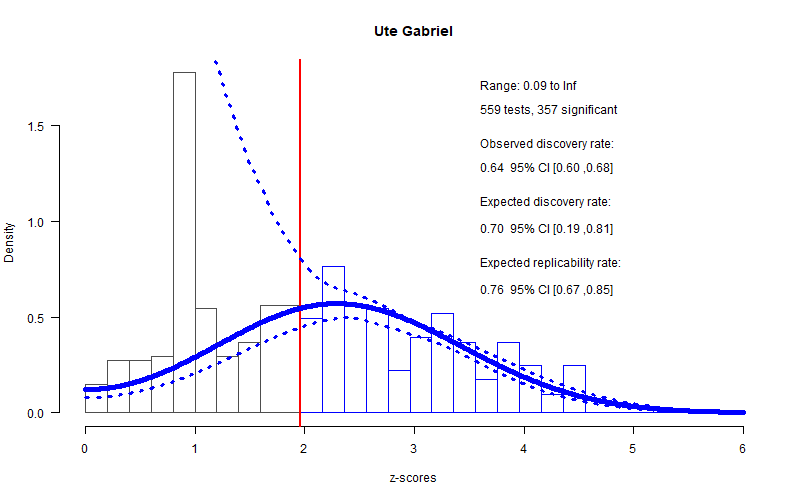
\includegraphics[width=\textwidth]{images/Ute Gabriel.png}
    \caption{z-verdier for Ute Gabriel}
\end{figure}
Ute Gabriel har en relativt flat graf, og ingen synlig diskontinuetet. Forventet replikasjonrate på 76\% er også ganske bra.

\subsection{Vera Skalicka}
\begin{figure}[h!]
    \centering
    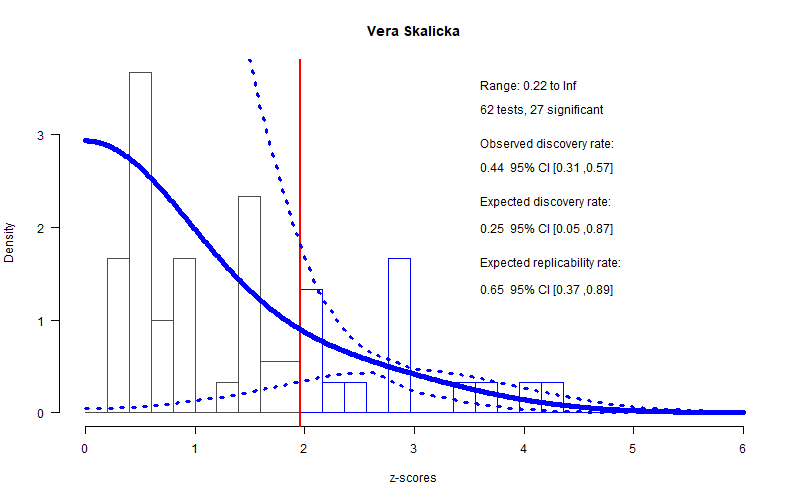
\includegraphics[width=\textwidth]{images/Vera Skalicka.png}
    \caption{z-verdier for Vera Skalicka}
\end{figure}
Vera Skalicka har ikke så mange resultater så vanskelig å si så mye ut fra grafen. Er en god del nullresultater, så lite tyder på p-hacking eller publikasjonsbias. En forventet replikasjonrate på 65\% er ganske OK.

\subsection{Xi Chu}
\begin{figure}[h!]
    \centering
    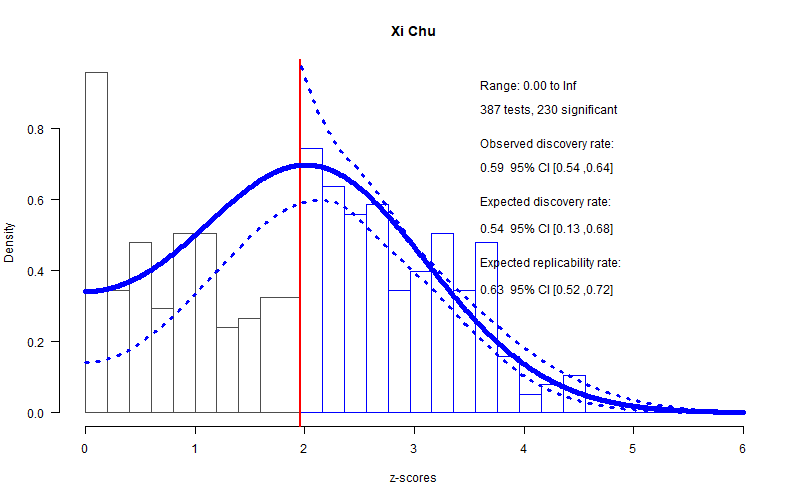
\includegraphics[width=\textwidth]{images/Xi Chu.png}
    \caption{z-verdier for Xi Chu}
\end{figure}
Xi Chu har en noe lav forventet replikasjonsrate på 63\%. Det er noe diskontinuetet ved $z=1.96$, selv om det også er publisert en god del nullresultater.

\subsection{En kommentar om forventet replikasjonrate}
Som vi så i første avsnitt er den empiriske replikasjonsraten i psykologi lav (et sted rundt 50\% eller mindre). Likevel har de aller fleste som er nevnt ovenfor her en replikasjonrate på greit over 50\%! Derfor kan det være verdt å merke seg at sammenligning mellom forventet replikasjonsrate og empirisk replikasjonsrate tilsier at forventet replikasjonrate slik som den er regnet ut her er ofte høyere enn replikasjonraten i praksis, så det er fort at forskerne over vil replikeres sjeldnere enn det statistikken over tilsier \parencite{z-curve-implementasjon, z-curve-mot-empiri}. \textcite{arp} bruker et gjennomsnitt mellom ERR og EDR kalt \guillemetleft Actual Replicability Prediction\guillemetright\ (ARP) som sin beste prediksjon på utfall av replikasjonsstudier. Som man kan se fra grafene over vil et ARP være noe lavere enn ERR som er brukt som forventet replikasjonrate i denne artikkelen.

\subsection{Så hvem vant?}
Det var mange her som har gjort en god innsats i å skulle bli instituttets beste p-hacker. Likevel var det ingen som hadde en så god diskontinuetet på $z=1.96$ som Frederikus Van der Weel. Han vant dermed konkurransen om å være instituttets beste p-hacker. Gratulerer!

\subsection{Mangler vi din yndlingsforsker?}

Mangler vi din yndlingsforsker (deg selv?) i denne artikkelen? Det er i såfall fordi vi ikke hadde nok p-verdier til å kunne få noe nyttig ut av en slik graf.

\subsection{Disclaimer}
P-verdiene ble hentet ut ved hjelp av et dataprogram, det fører til at noe av p-verdiene fra artikler mangler siden programmet ikke klarer å hente ut alle p-verdiene. Det kan være at noen er hentet ut feil. En diskontinuetet i en z-verdi-graf trenger ikke å bety at man har gjort noe uetisk i forskningen sin eller at man har drevet med p-hacking, men heller at man har større sjanse for å nevne statistiske resultater på signifikante resultater, mens nullresultater beskrives kvalitativt og vil dermed ikke bli regnet med her. Den forventede replikasjonraten er en statistisk verdi utregnet fra p-verdiene, og er ikke sikkert samsvarer med en faktisk replikasjonrate på studiene. Når forventet replikasjonrate er nevnt hos forskere i artikkelen er det fokus på den estimerte verdien, men konfidensintervallet er stort. Mange med \guillemetleft gode\guillemetright\ forventede replikasjonrater har også ganske \guillemetleft dårlige\guillemetright\ forventede replikasjonrater i 95\% konfidensintervallet sitt og vica versa. Så den kvalitativte beskrivelsen av replikasjonratene i teksten baserer seg ofte ikke på statistisk signifikante forskjeller. Om noen av forskerene har gitt ut få artikler kan også det føre til at z-verdi-grafen ikke er særlig god.

\printbibliography

% Ta alle bilder til slutt fordi det er det layout i Psykologisk Tidsskrift jobber ut fra
\processdelayedfloats

\end{document}